\documentclass[12pt]{article}
\usepackage[left=1in,right=1in,top=1in,bottom=1in]{geometry}
\usepackage{enumerate}
\usepackage{graphicx}
\usepackage{amsmath}
\usepackage{amssymb}
\usepackage{amsfonts}
\usepackage{amsthm}
\usepackage{enumerate}
\usepackage{url}
\usepackage{color}
\usepackage{listings}
\usepackage{wasysym}
\usepackage{tikz}
\usetikzlibrary{matrix,arrows}

\def\class{CS 5220}
\def\date{11/14/2011}
\def\prof{Professor Bindel}
\def\name{tbe4, dsj36}
\def\title{Project \#3: All Pairs Shortest Paths}
\usepackage{setspace}
\onehalfspacing

\usepackage{fancyhdr}
\pagestyle{fancy}
\lhead{\class\\\name}
\rhead{\title\\\date}

\newtheorem{lemma}{Lemma}
\def\R{\mathbb{R}}
\def\F{\mathbb{F}}
\def\C{\mathbb{C}}
\def\N{\mathbb{N}}
\def\Q{\mathbb{Q}}
\def\Z{\mathbb{Z}}
\def\C{\mathbb{C}}
\def\a{\alpha}
\def\b{\beta}
\def\d{\delta}
\def\e{\varepsilon}
\def\w{\omega}
\def\Span{\text{Span}}
\def\char{\text{char}}
\def\im{\text{im}}
\def\Hom{\text{Hom}}
\def\deg{\text{deg}}

\newcommand{\hwproblem}[2]{
\vspace{1em} \noindent{\bf #1} #2} % \vspace{1em}}
\newcommand{\hwheading}{
\thispagestyle{empty} \noindent
   \begin{center}
   \framebox{
      \vbox{
    \hbox to 5.78in { \large {\bf \class}
         \hfill \date }
       \vspace{4mm}
       \hbox to 5.78in { {\Large \hfill \title  \hfill} }
       \vspace{2mm}
       \hbox to 5.78in { \large {\it \prof \hfill \name} }
      }
   }
   \end{center}
}
\newcommand{\hwsolution}[1]{\vspace{1em} \noindent {\emph{#1.}}}

\lstset{
  basicstyle=\footnotesize,
  language=C,
  frame=single
}

\begin{document} \hwheading

\subsection*{Introduction}

Given a graph specified by an adjacency matrix, the Floyd-Warshall
algorithm computes a matrix $A$ where $A_{ij}$ is the length of the
shortest path from node $i$ to node $j$. This algorithm computes the
shortest path between each pair of nodes at once, but it does not tell
us anything else about the paths.  Using the dynamic programming idea,
we have the following recurrence, where $A_{ij}^s$ is the length of
the shortest path of at most $2^s$ steps.
\[ A_{ij}^{s+1} = \min _k \{ A_{ik}^s + A_{kj}^s \} \] Therefore, we
may start with $s = 0$, which corresponds to the adjacency matrix of
the graph with the distance of unconnected vertices set to infinity,
and iterate until we reach a fixed point. Since we are working with
unweighted edges, we do not have to worry about negative cycles. Once
we are done iterating, we set the edges of distance infinity to zero
to return to the adjacency matrix representation.

\subsection*{Reference Implementation}
The reference implementation of this algorithm is a straightforward
parallelization in OpenMP. The loop over the columns, indexed by {\tt
j}, is split among the threads with an {\tt omp parallel}
pragma. After compiling with the {\tt -O3} optimization flag, the
scaling of this implementation was quite passable. We ran the program
on randomly generated graphs of sizes 50 to 2000 nodes in steps of 50.
Here is the data from the weak scaling study in both linear and
log-log plots.

\begin{figure}
  \centering
  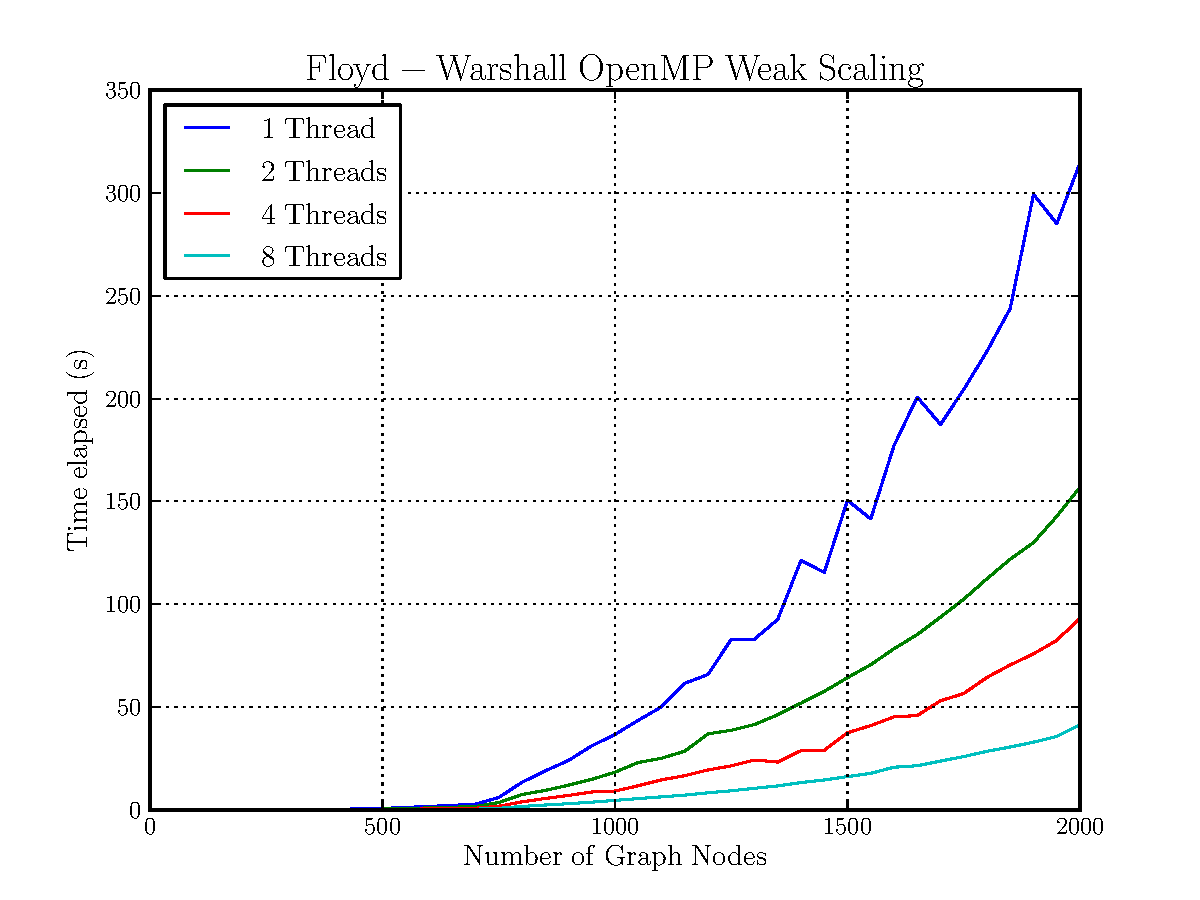
\includegraphics[scale=0.7]{../profiling/omp_linear_weak.pdf}
  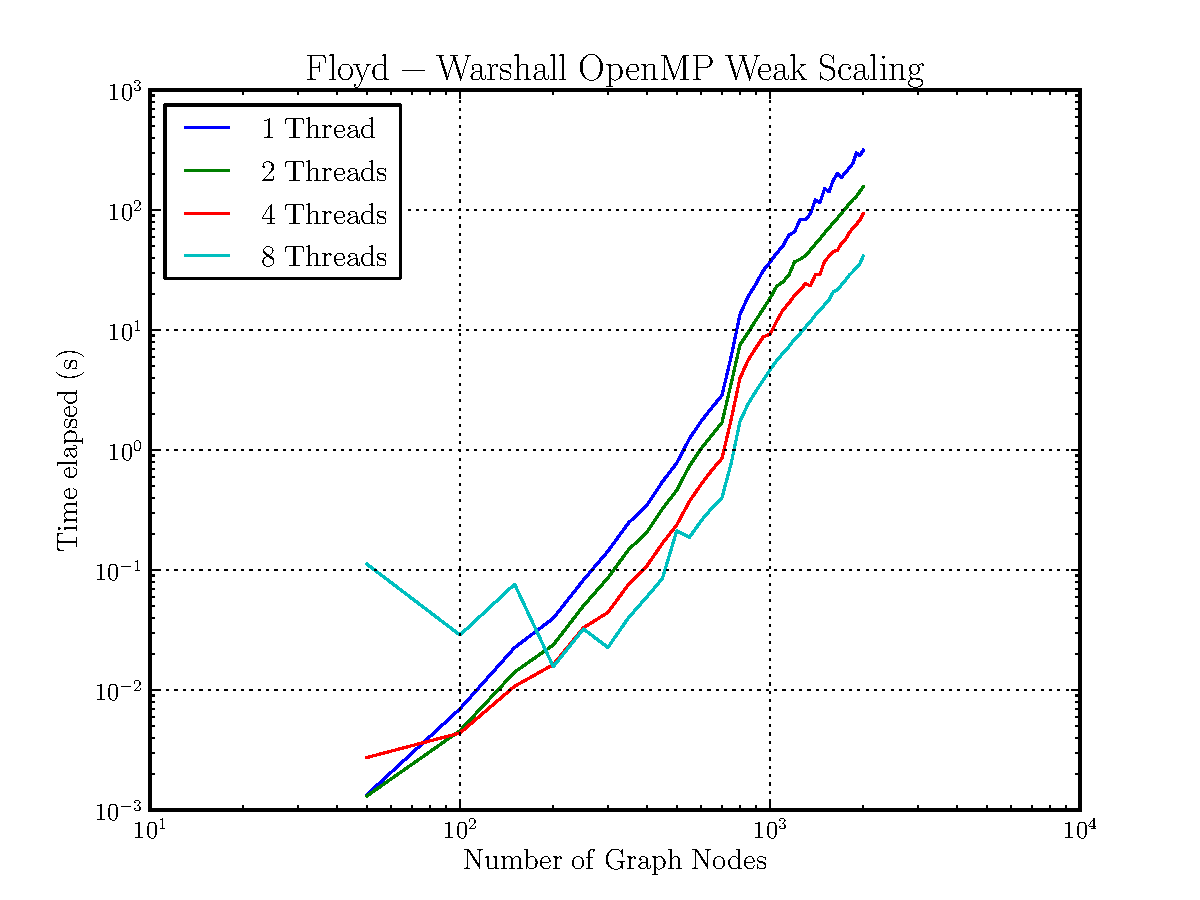
\includegraphics[scale=0.7]{../profiling/omp_log_weak.pdf}
  \caption{Weak scaling results from the reference OpenMP implementation}
\end{figure}

From the logarithmic plot, we observe that as the number of nodes
becomes large, the slope of the plot roughly settles to around three,
as we would expect from the $O(n^3 \log n)$ asymptotic behavior of our
algorithm. Curiously, the number of iterations needed per experiment
changed little. Past 200 nodes, each experiment used exactly three
iterations. The randomly generated graph of 50 nodes required five
iterations, the most of any graph.

Similarly, we fixed the problem size at 2000 nodes and varied the
number of OpenMP threads from one to eight to collect data for the
strong scaling experiment. The ratio between the time taken with one
thread is plotted below.

\begin{figure}[h!]
  \centering
  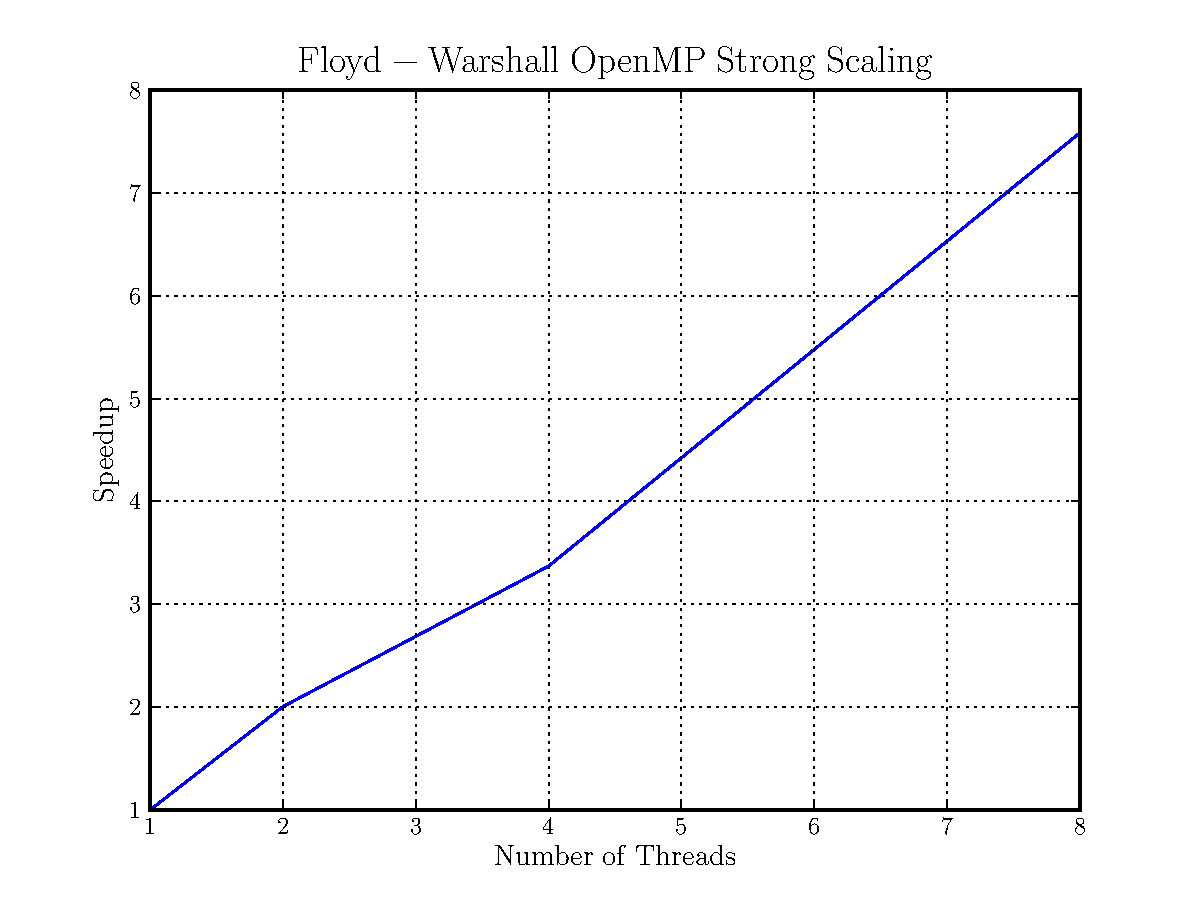
\includegraphics[scale=0.7]{../profiling/omp_strong.pdf}
  \caption{Strong scaling results from the reference OpenMP implementation}
\end{figure}

\noindent The OpenMP codes scale just below the $p$ times speedup, which
is good. Furthermore, we were not able to improve on the asymptotic
behavior of the code, as the algorithm itself is $O(n^3 \log n)$. However,
we were able to significantly improve the constant factor with some
optimizations.

\vspace{0.75em}
\noindent We profiled the OpenMP implementation with HPC Toolkit,
but we found that after providing {\tt gcc} the {\tt -O3} optimization
flag, the profiler did not give us much useful data. Specifically, almost
all our time was reported spent in the comparison between the $l_{ik}$ and
$l_{kj}$ and $l_{ij}$ distances, which makes sense as it is the main
computation in our inner loop. We were not able to diagnose any bottlenecks
with the profiler.
\noindent

\subsection*{Naive MPI Implementation}

Since it does not rely on shared memory access, MPI is natural choice for
improving the scaling of the code units. Our first implementation simply maintains
a full copy of the distance matrix at each thread and synchronizes after
each iteration with an {\tt MPI\_AllGatherv} command. As expected, each thread
must broadcast its columns of the matrix to every other thread, incurring
a roughly $O(n^2)$ cost. Our main aim in the remainder of this project will
be to decrease the constant factor of these communication costs.

\vspace{0.75em}
\noindent We collected similar data on the performance of the naive implementation.
Given the amount of communication needed, it is no surprise that the naive code
did not scale well.

\begin{figure}[h!]
  \centering
  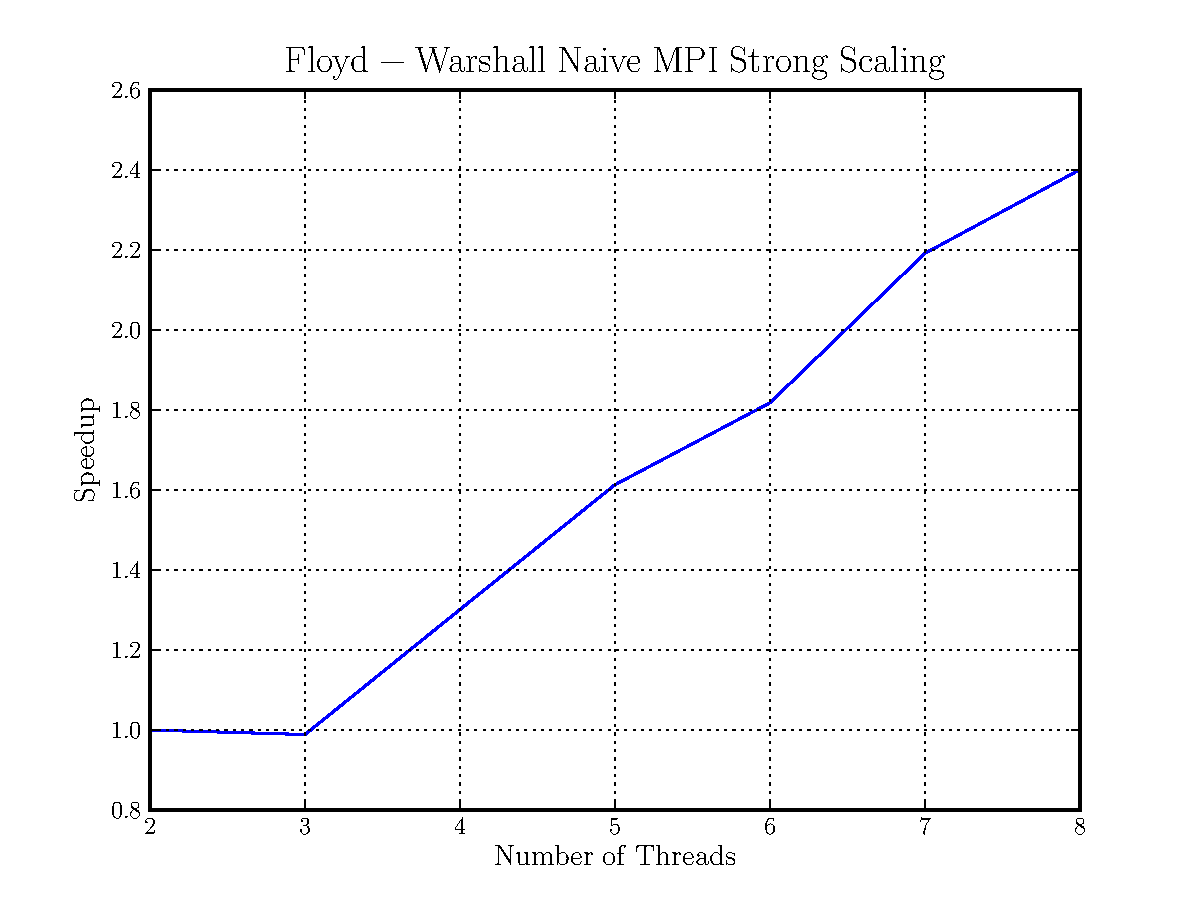
\includegraphics[scale=0.7]{../profiling/naive/naive_strong.pdf}
  \caption{Strong scaling results from the naive MPI implementation. Note
    that running our code with eight threads is only a modest improvement
    over running it with two threads.}
\end{figure}

\begin{figure}[h!]
  \centering
  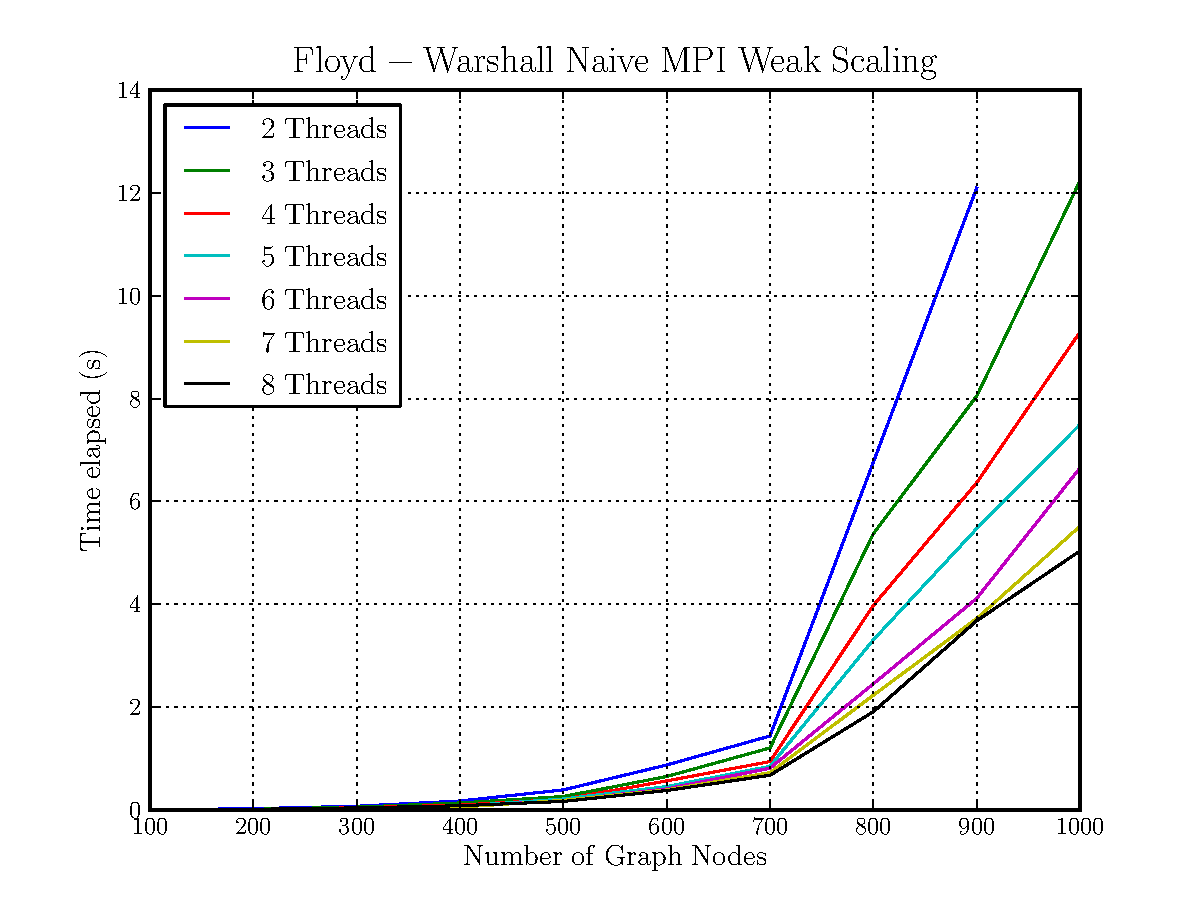
\includegraphics[scale=0.7]{../profiling/naive/naive_linear_weak.pdf}
  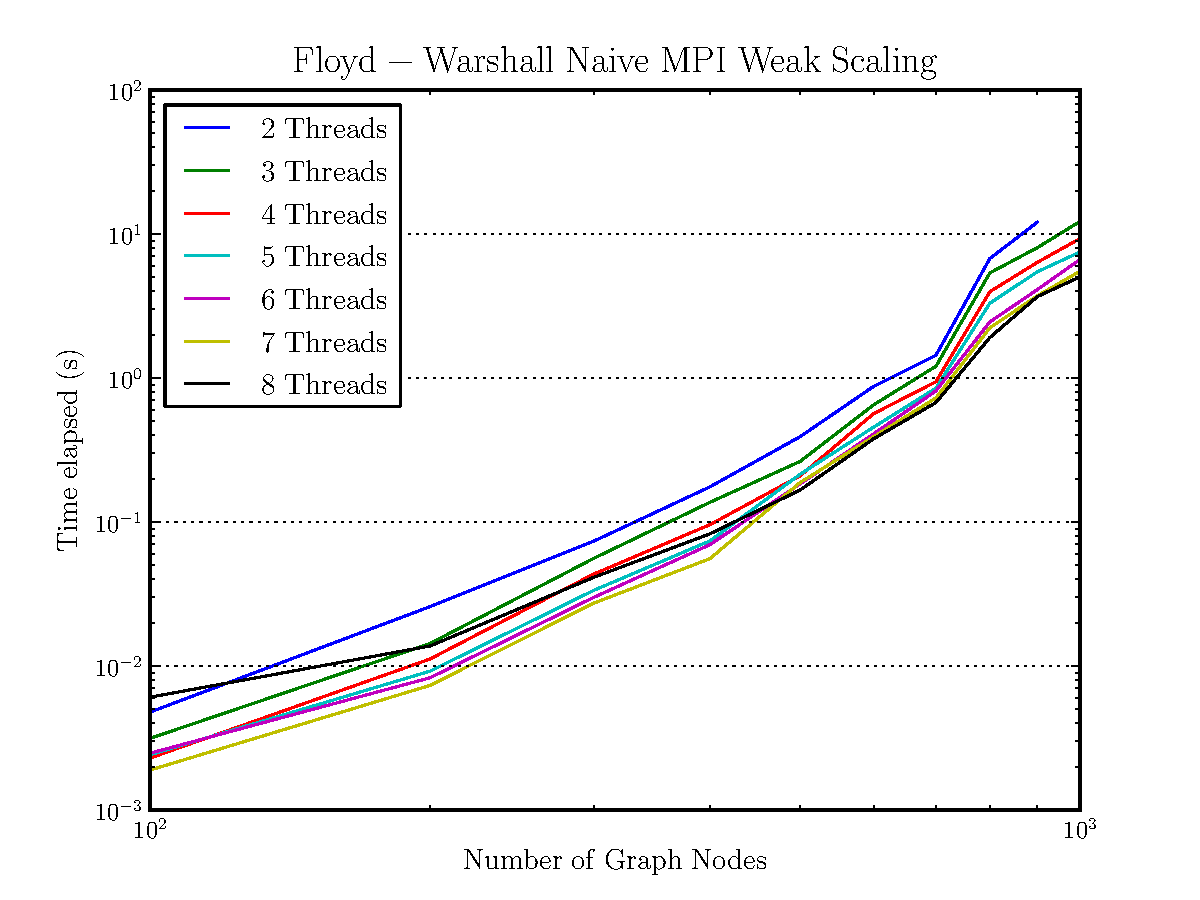
\includegraphics[scale=0.7]{../profiling/naive/naive_log_weak.pdf}
  \caption{Weak scaling results from the naive MPI implementation. Note that
    in the log-log plot, the curves are only displaced vertically from each
    other by a small amount:  This indicates that the constant factor of
    improvement is not much from increasing the number of threads.}
\end{figure}

\subsection*{Ring MPI Implementation}

The main idea behind this project is that we can rearrange the recurrence
so that each thread only needs to see a few columns at once. Therefore,
we may pass the columns of the original matrix around round-robin style,
incurring much less communication overhead. Note, however, that our asymptotics
do not improve, as $O(n^2 / p)$ entries still need to be communicated.

\vspace{0.75em}
\noindent Let $\{ c_1, c_2, \ldots, c_p \}$ indicate a partition of the columns
among the processors, and rewrite the recurrence as follows.
\[ A_{ij}^{s+1} = \min \left\{ \min_{k=0}^{c_1} \{ A_{ik}^s + A_{kj}^s \},
\ldots,
\min_{k=c_p}^{n} \{ A_{ik}^s + A_{kj}^s \} \right\}\]
That is, we may compute the minima over only a few $k$, which correspond
to columns of the matrix, and then keep a running minimum in our final
matrix. The communication pattern starts with each thread doing the computations
that involve only its local columns. Each thread then passes its chunk
of columns to the right and receives from the left, wrapping around if
needed. The computations involving these columns are then performed, and
the process continues until each thread has seen every column. We maintain
a flag on each thread indicating whether any of its columns have changed and
then use {\tt MPI\_Allreduce} to determine whether all the threads have
completed.

\vspace{0.75em}
\noindent As we would hope, the performance of this implementation was an
improvement. We ran the usual set of strong and weak scaling experiments
on this implementation as well.

\begin{figure}
  \centering
  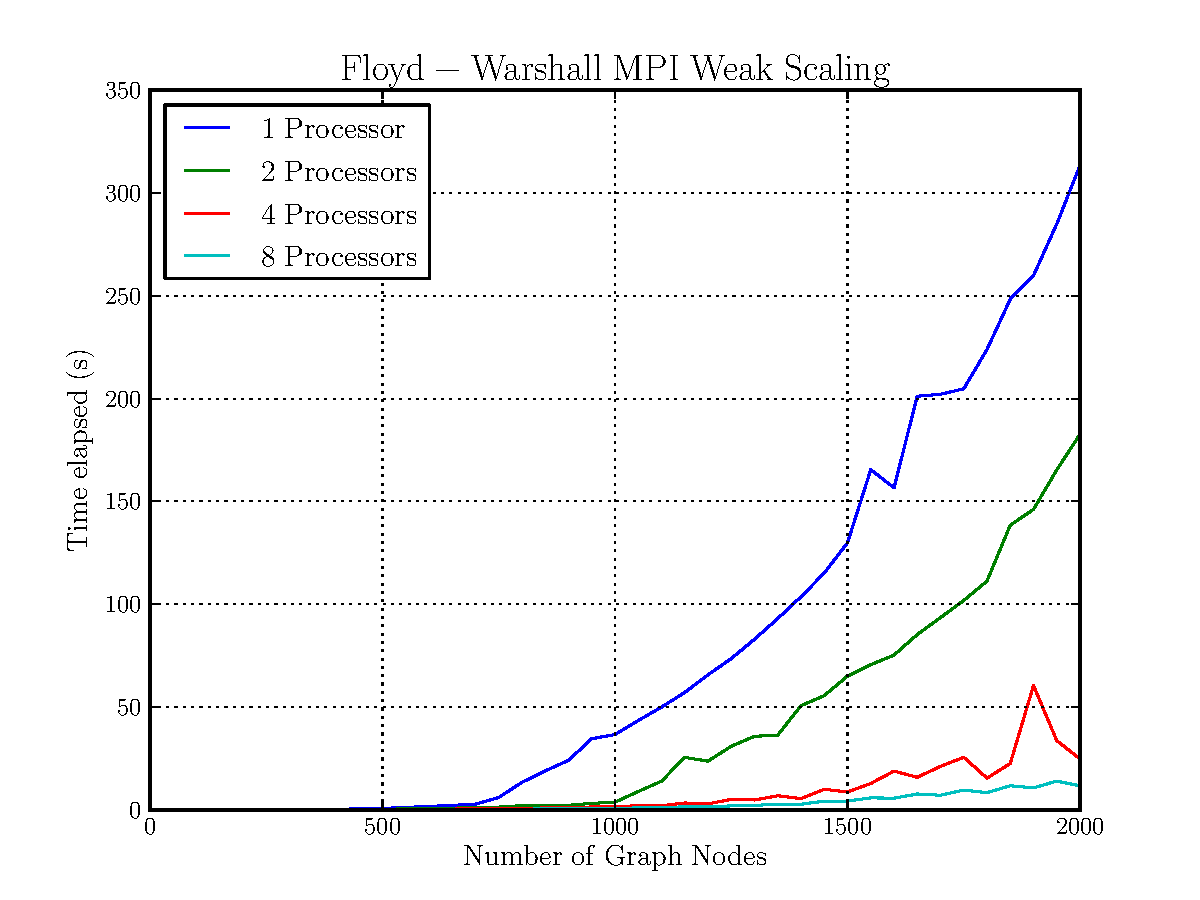
\includegraphics[scale=0.7]{../profiling/mpi_linear_weak.pdf}
  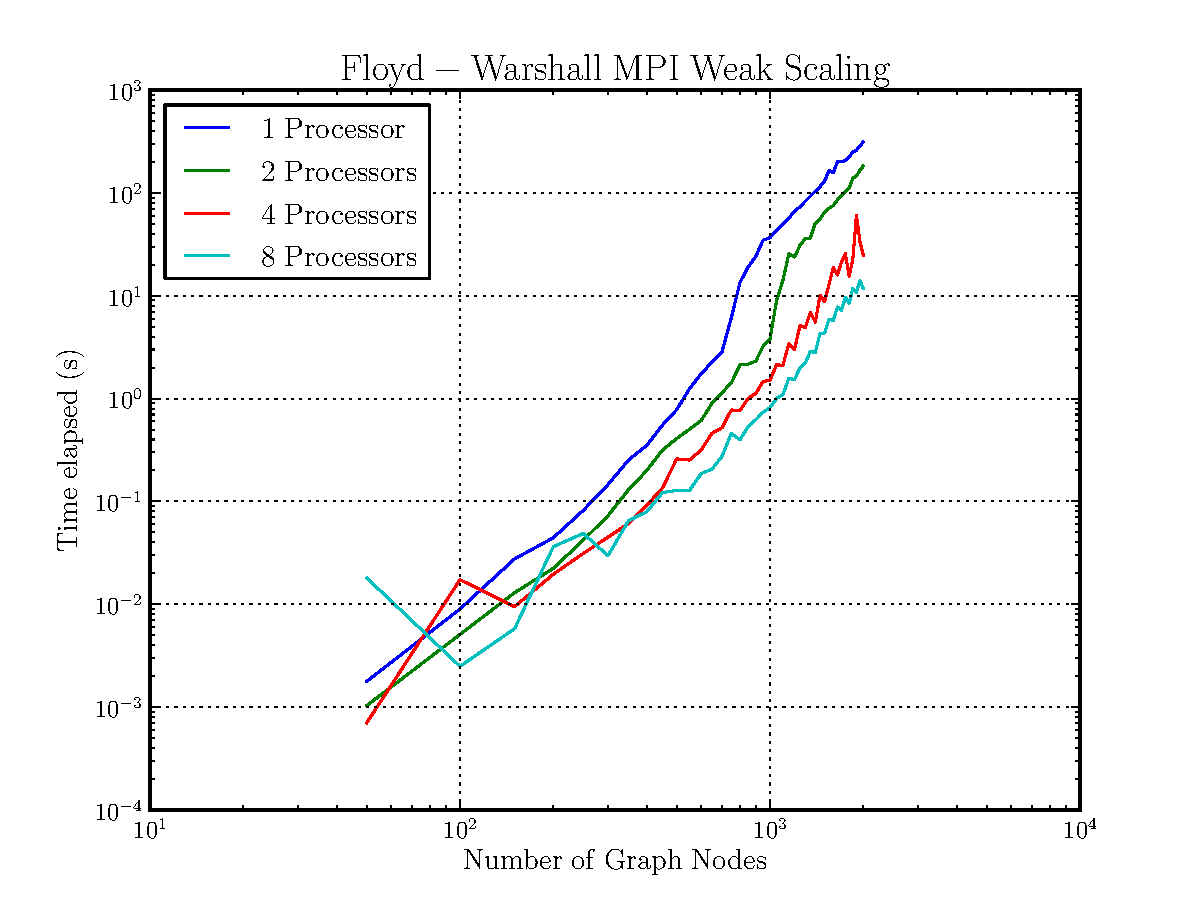
\includegraphics[scale=0.7]{../profiling/mpi_log_weak.pdf}
  \caption{The usual weak scaling experiments for the optimized MPI
    implementation. The log-log plot shows a good improvement in the
    constant factor with increased processor count, but, as expected,
    the asymptotic behavior remains the same.}
\end{figure}

\begin{figure}
  \centering
  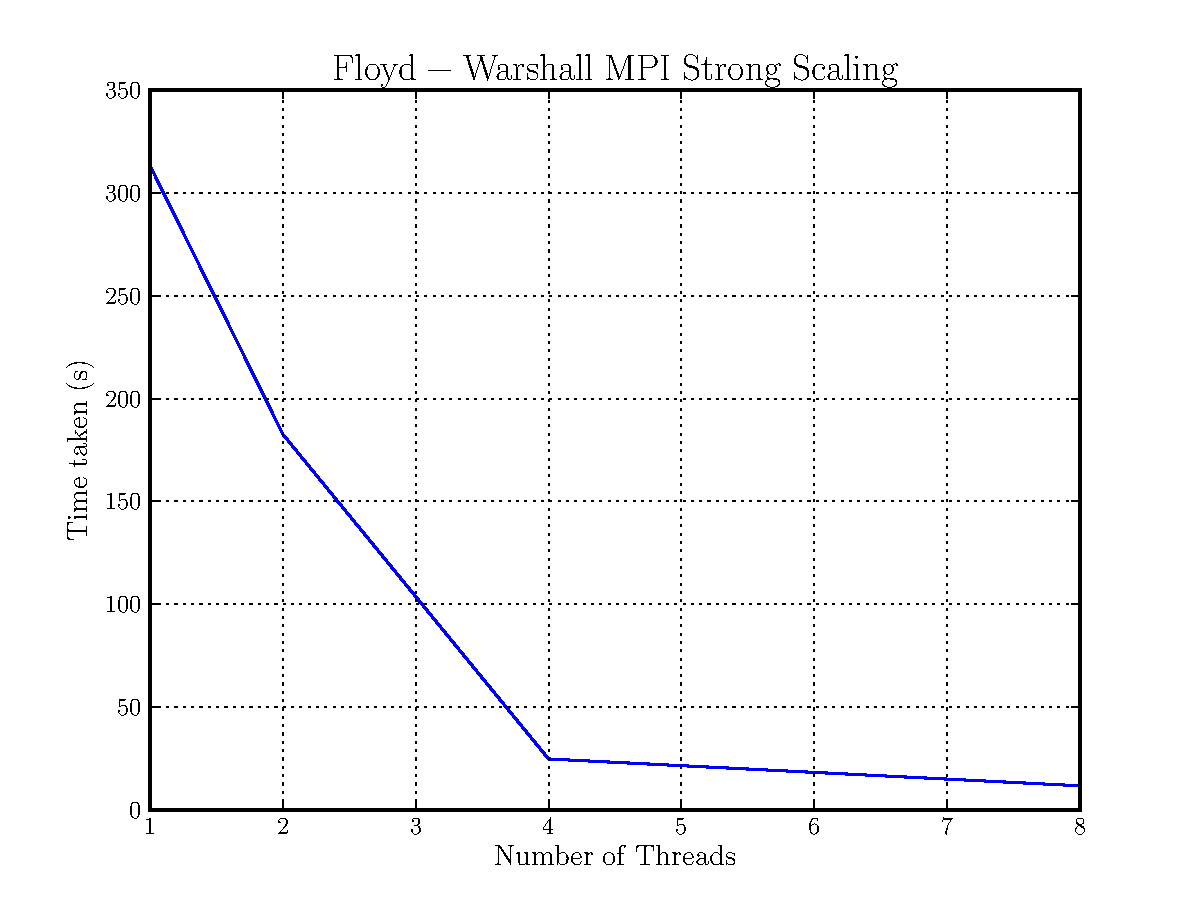
\includegraphics[scale=0.7]{../profiling/mpi_strong.pdf}
  \caption{This strong scaling plot is a little misleading. There
    is a significant amount of overhead when we run the code with
    a few number of processors, so the 25 times speedup with eight
    processors isn't quite genuine.}
\end{figure}

\noindent In addition, we manually instrumented our code to determine the
amount of time spent in communication versus computation. We simply used
{\tt MPI\_Wtime()} before and after the major computation and communication
events and kept a running total of the time spent in each section.

\begin{figure}
  \centering
  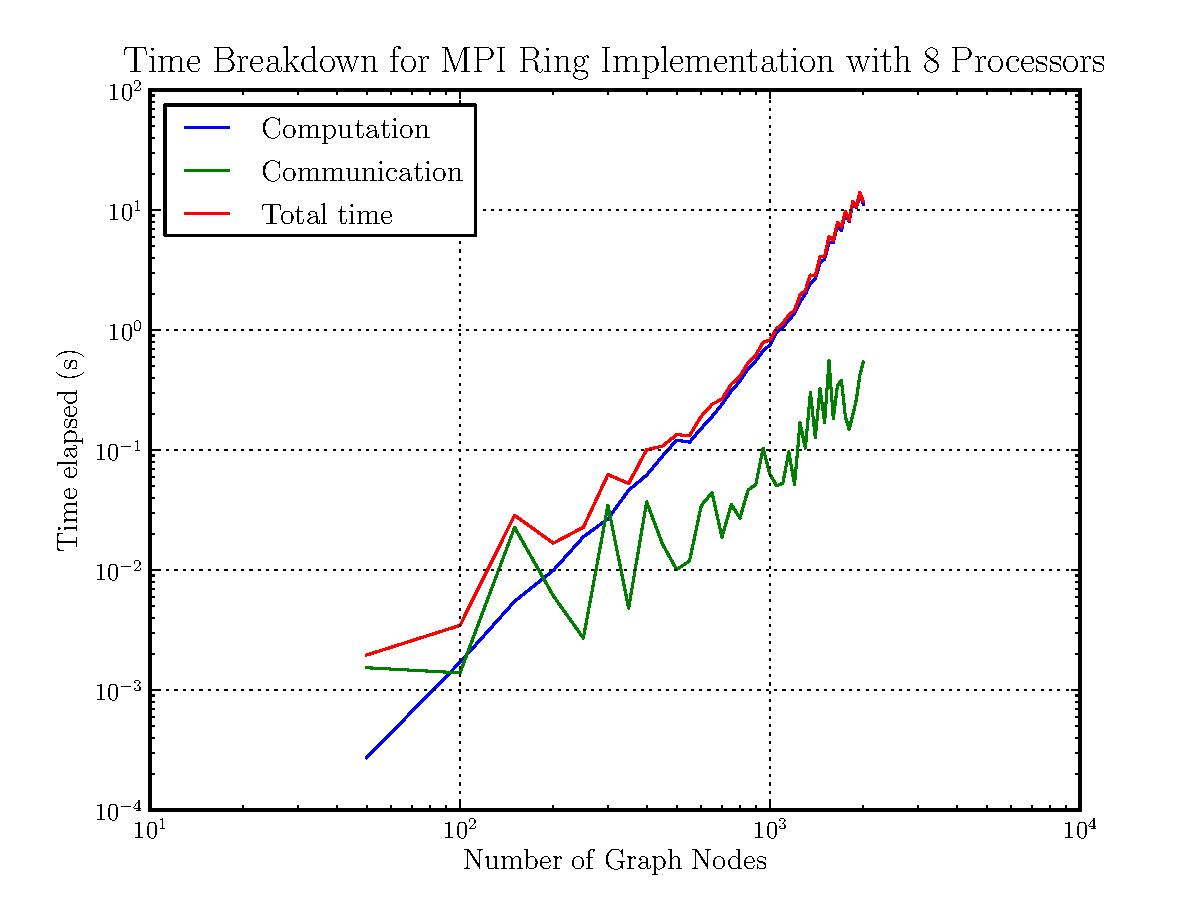
\includegraphics[scale=0.7]{../profiling/mpi_log_timing_8.pdf}
  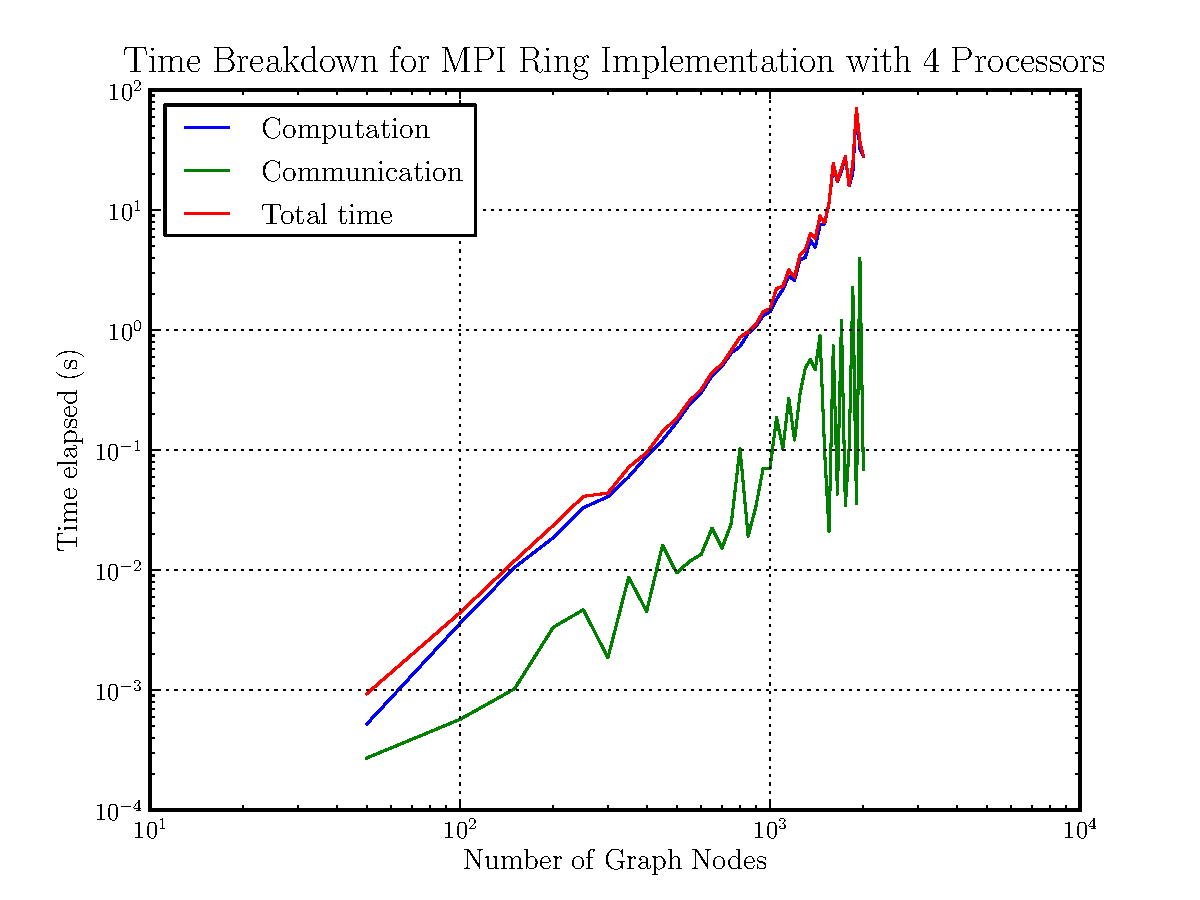
\includegraphics[scale=0.7]{../profiling/mpi_log_timing_4.pdf}
  \caption{Breakdown of time spent in computation and communication on a
    log-log plot for the ring MPI implementation.}
\end{figure}

\vspace{0.75em}
\noindent The communication time is almost an order of magnitude smaller than the
computation time once we have a sufficiently large graph. However,
note that the slope of the communication curve is still two, indicating
a quadratic amount of communication. This result stems from our previous
observation that we did not actually improve the asymptotic behavior
of the code.

\vspace{0.75em}
\noindent In terms of explaining the communication costs in terms
of, say, the $\alpha-\beta$ model, the linear factors for latency and
bandwidth are hidden behind the quadratic behavior of the communication
time. However, the results from our manual profiling do confirm our suspicions
that the computation is indeed $O(n^3 \log n)$ and the communication is
$O(n^2)$.

\vspace{0.75em}
\noindent We conclude with some comparisons between the OpenMP and ring MPI
implementations. For large graphs, the MPI implementation is about two times
faster than the OpenMP implementation.

\begin{figure}
  \centering
  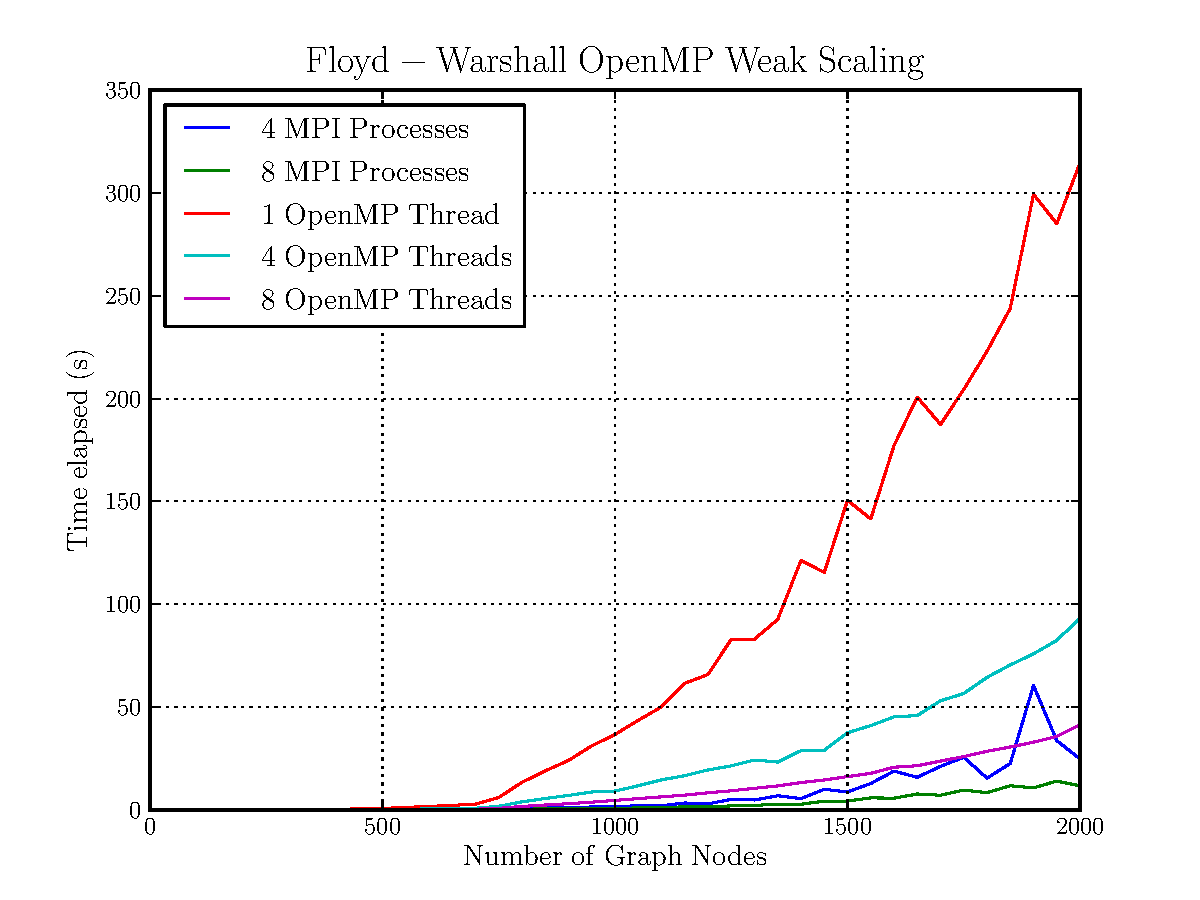
\includegraphics[scale=0.7]{../profiling/linear_comparison.pdf}
  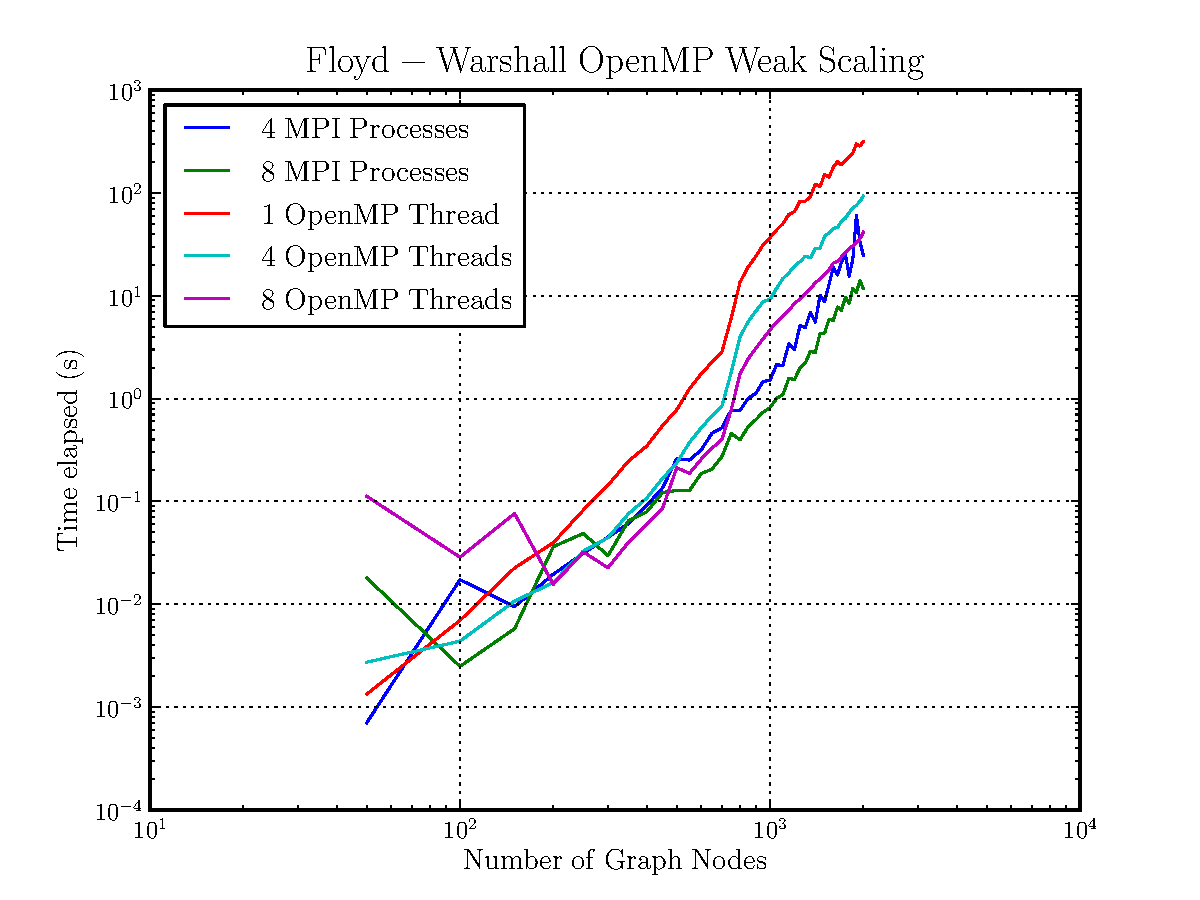
\includegraphics[scale=0.7]{../profiling/log_comparison.pdf}
  \caption{A comparison of our timing experiments for the optimized
    MPI and OpenMP implementations. Note that the fastest MPI code
    runs roughly twice as fast as the OpenMP code for large graphs.}
\end{figure}

\end{document}
